\documentclass[../../ASSD_TP1_G7.tex]{subfiles}
\begin{document}
\chapter*{Mediciones b\'asicas}
Para esta sección del informe, vamos a proceder a tomar las mediciones
pertinentes al punto 6 del trabajo práctico, las cuales constan de
varias mediciones progresivas sobre la placa total ya ensamblada.
Las configuraciones de la placa para la cual se realizaron las mediciones
son, a saber:
\begin{itemize}
\item Muestreo natural: FAA + llave analógica + FR~
\item Muestreo con Sample and Hold: FAA + S\&H + FR
\end{itemize}
Para cada caso, se emplearán dos funciones $X_{a}$ y $X_{b}$ siendo
$X_{a}=A\cdot Cos(2\cdot\pi\cdot f_{in}\cdot t)$ y $X_{b}=funci\acute{o}n\,rampa$.

Aplicando dichas señales, se midieron los siguientes items:
\begin{enumerate}
\item Salida proporcional a la entrada con la menor distorsión posible,
optimizando $f_{s}$, A y el duty cycle del oscilador; y hallar el
porcentaje de potencia recuperada.
\item Igual que el insciso 1 pero con nuevos valores para $f_{in}\leq\frac{f_{p}}{2}$,
con $f_{s}=f_{a}$; y con $f_{in}=f_{a}$ y $f_{s}$variable.
\item Ingreso con $f_{in}=f_{s}\leq f_{p}$ y justificar matemáticamente
lo observado. (Solo para $X_{a}$)
\item Variar su frecuencia hasta que comiencen a manifestarse problemas
de alias a la salida del FAA. (Solo para $X_{b})$
\end{enumerate}

\section{Mediciones con la llave analógica}

\subsection{Placa optimizada}

Para estas mediciones, se calibraron todas las partes de la placa
par así poder obtener la menor distorción posible con un óptimo $f_{s}\,y\,A$.
Podemos observar el resultado en las siguientes imágenes:

\begin{figure}[H]

\centering{}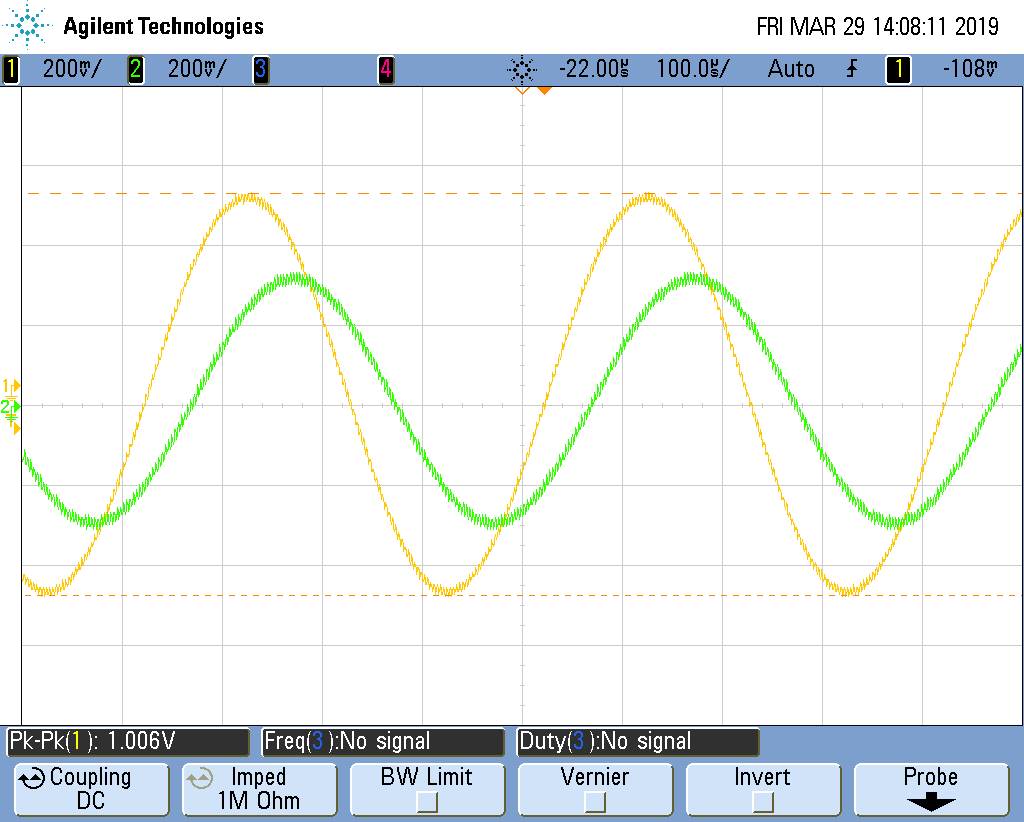
\includegraphics[scale=0.25]{Imagenes/llave_senooo_pto_a1}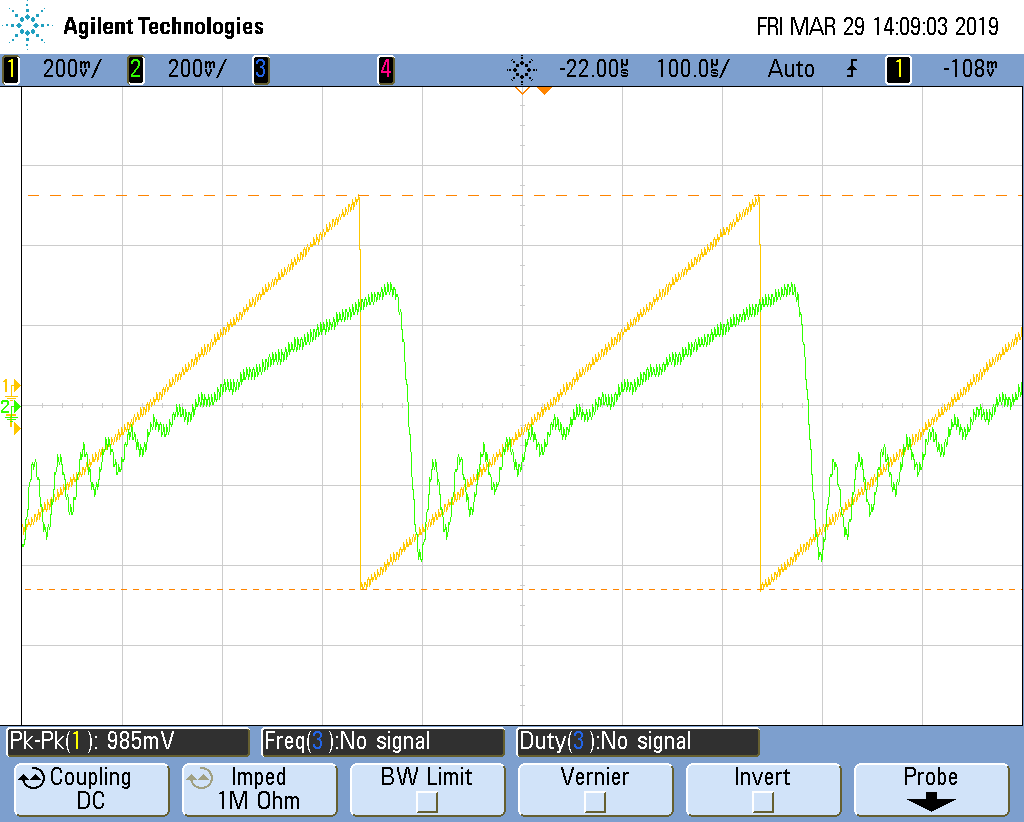
\includegraphics[scale=0.25]{Imagenes/llave_diente_pto_a}\caption{De izq a der: salida (verde) de la placa con $X_{a}$; salida con
$X_{b}$}
\end{figure}

Para la señal $X_{a}$, los valores óptimos que se obtuvieron fueron:
$f_{s}:[76,3;313](kHz)$midiendo en el máximo de ese intervalo, $DC=48.5\%,$$A:(0;2]$(Vpp)
midiendo para $A=1V_{pp}$.

Para la señal $X_{b}$, los valores óptimos obtenidos fueron: $f_{s}:[91;313](kHz)$midiendo
en el máximo de ese intervalo, $DC=48.8\%,$$A:(0;2]$(Vpp) midiendo
para $A=1V_{pp}$.

FALTA POTENCIA Y DESARROLLO MATEMATICO???

\subsection{Cambios en la $f_{in}$ y en la $f_{s}$}

\subsubsection{$f_{in}<\frac{f_{p}}{2}$,$f_{s}=f_{a}$}

Para este caso, se exitó a la placa con una señal $X_{a}$, con la
diferencia respecto al punto anterior de que ahora el rango de $f_{in}=(0;45]$(kHz)
y la $f_{s}=68kHz.$Con el nuevo intervalo de $f_{in}$, finalmente
se eligió $f_{in}=500Hz.$ El duty cycle utilizado fue de 47.6\%.

Para la señal $X_{b}$, por otra parte el rango de $f_{in}$ pasó
a ser $f_{in}=(0;45]$(kHz) y la $f_{s}$ mantuvo su valor de $68kHz.$Con
el nuevo intervalo de $f_{in}$, finalmente se eligió $f_{in}=500Hz.$
El duty cycle utilizado también fue de 47.6\%.

Los resultados se ven plasmados en la siguiente image:

\begin{figure}[H]

\centering{}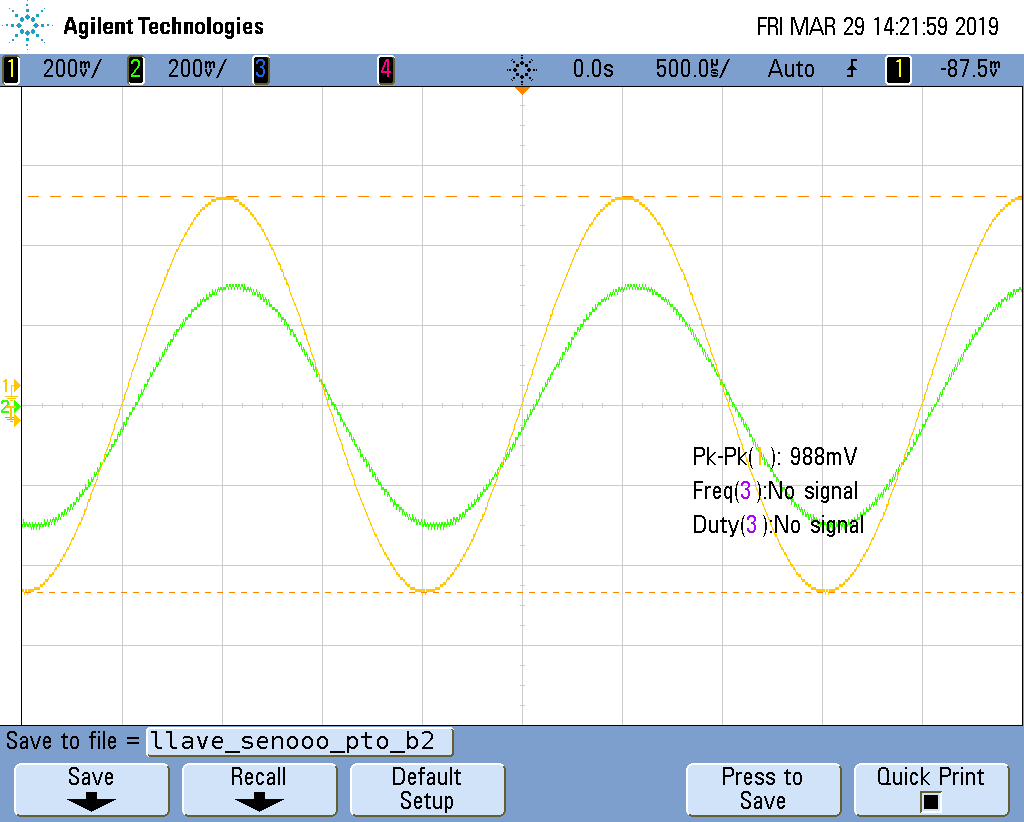
\includegraphics[scale=0.25]{Imagenes/llave_senooo_pto_b2}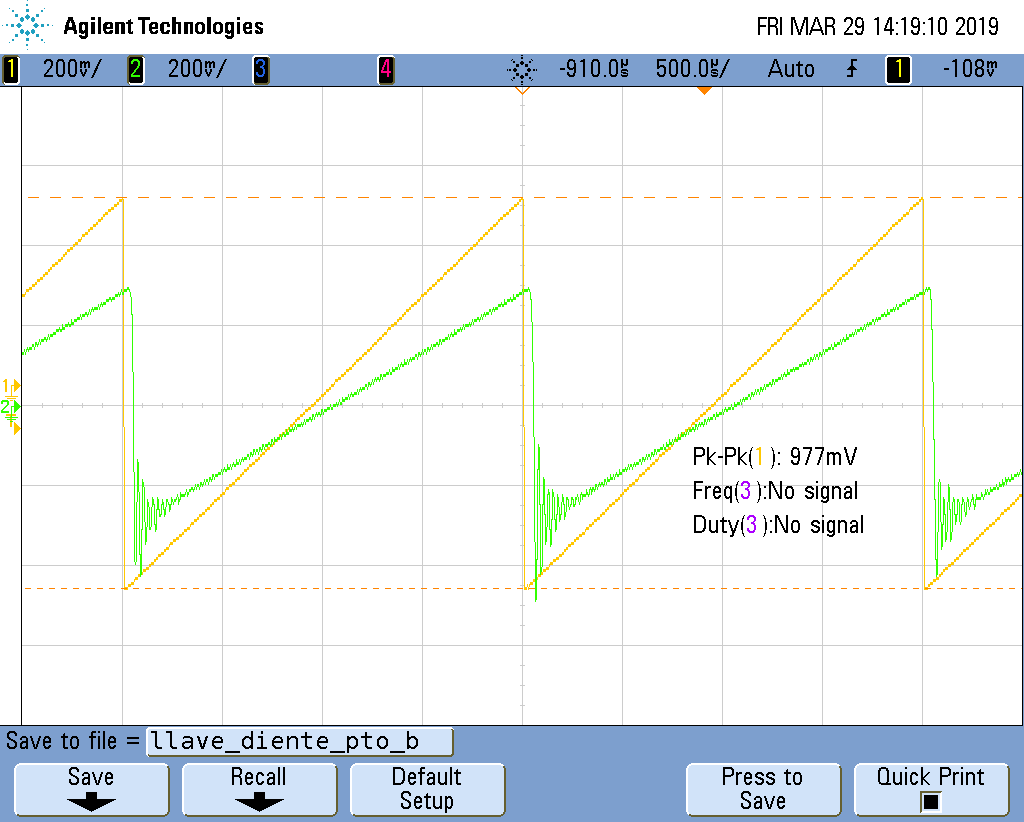
\includegraphics[scale=0.25]{Imagenes/llave_diente_pto_b}\caption{De izquierda a derecha: señal $X_{a}$y señal $X_{b}$.}
\end{figure}


\subsubsection{$f_{in}=f_{a}$}

Para este punto, tanto a la señal $X_{a}$ como $X_{b}$, se las estableció
con una frecuencia $f_{in}=68kHz$. Para la frecuencia de muestreo,
se optó por utilizar la máxima posible, es decir $f_{s}=313kHz.$Para
ambas señales, se mantuvo el mismo duty cycle de 48\%. Los resultados
pueden ser apreciados en la siguiente imagen:

\begin{figure}[H]

\begin{centering}
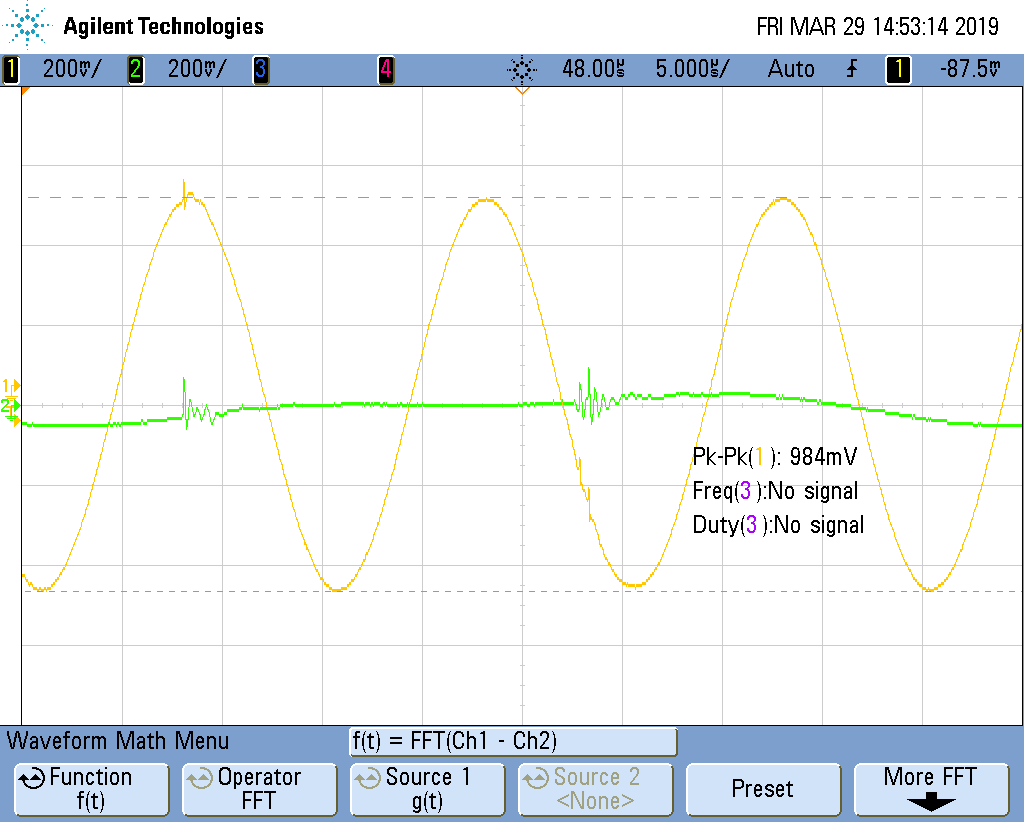
\includegraphics[scale=0.25]{Imagenes/llave_senooo_pto_bf1}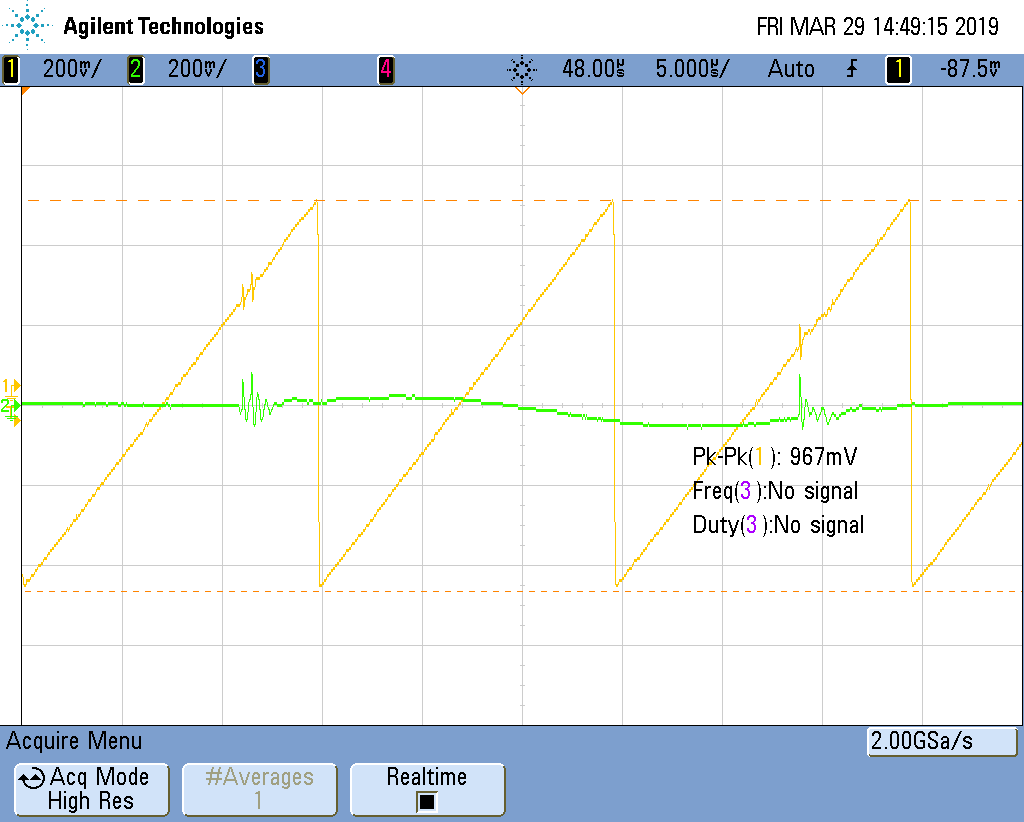
\includegraphics[scale=0.25]{Imagenes/llave_djente_pto_bfa}\caption{De izquierda a derecha: señal $X_{a}$y señal $X_{b}$.}
\par\end{centering}
\end{figure}


\subsection{$f_{in}=f_{s}\protect\leq f_{p}$}

Para este caso, solamente se exito al circuito con la señal $X_{a}$
con la particularidad que la frecuencia de la señal coincide con la
frecuencia de sampleo. Para ello, se optó por utilizar $f_{in}=f_{s}=10kHz$
y un DC de 47.3\%. La salida resultante se aprecia a continuación:

\begin{figure}[H]
\begin{centering}
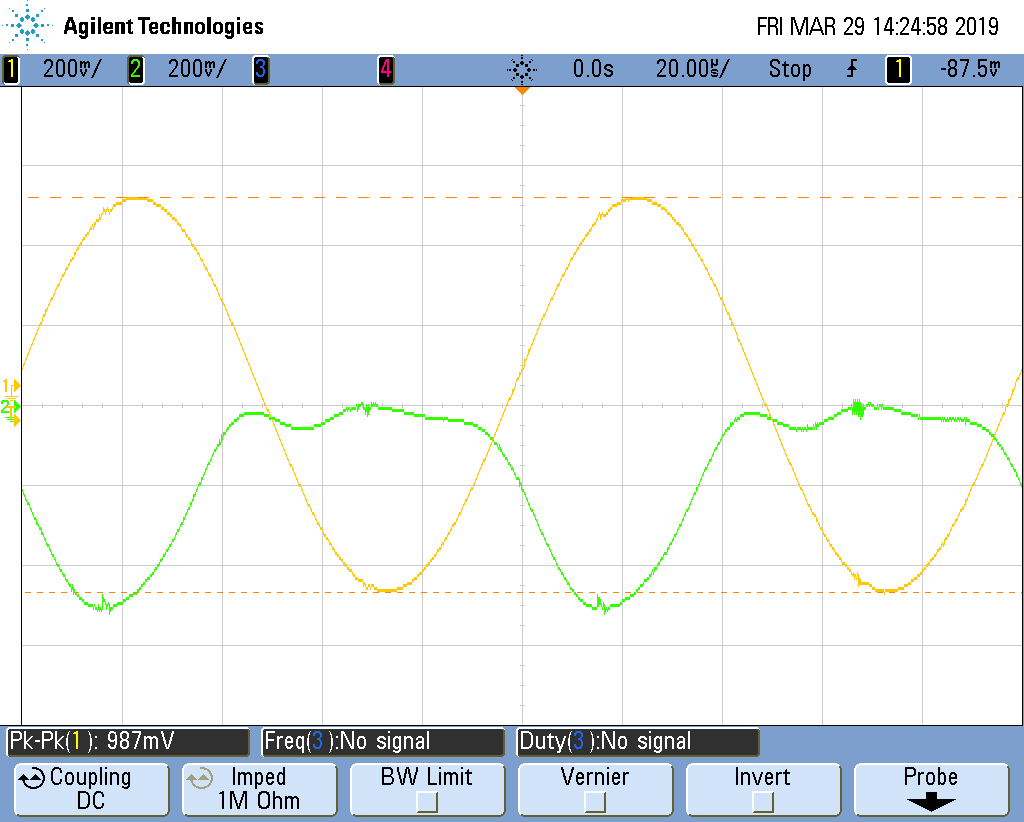
\includegraphics[scale=0.3]{Imagenes/llave_senooo_pto_c}\caption{Señal $X_{b}$ con frecuencia de muestreo igual a la de la señal.}
\par\end{centering}
\end{figure}


\subsection{Aliasing}

Para esta úlitma medición con la llave analógica, se exitó al circuito
con la señal $X_{b}$ variando su frecuencia $f_{in}$ de manera tal
de poder encontrar a qué frecuencia comienzan a aparecer problemas
de aliasing. Configurando la señal a una $f_{in}=2.5kHz,$observamos
que el efecto de aliasing aparece cuando la señal $f_{s}<45kHz$.
Podemos ver los efectos en la siguiente imagen:

\begin{figure}[H]
\begin{centering}
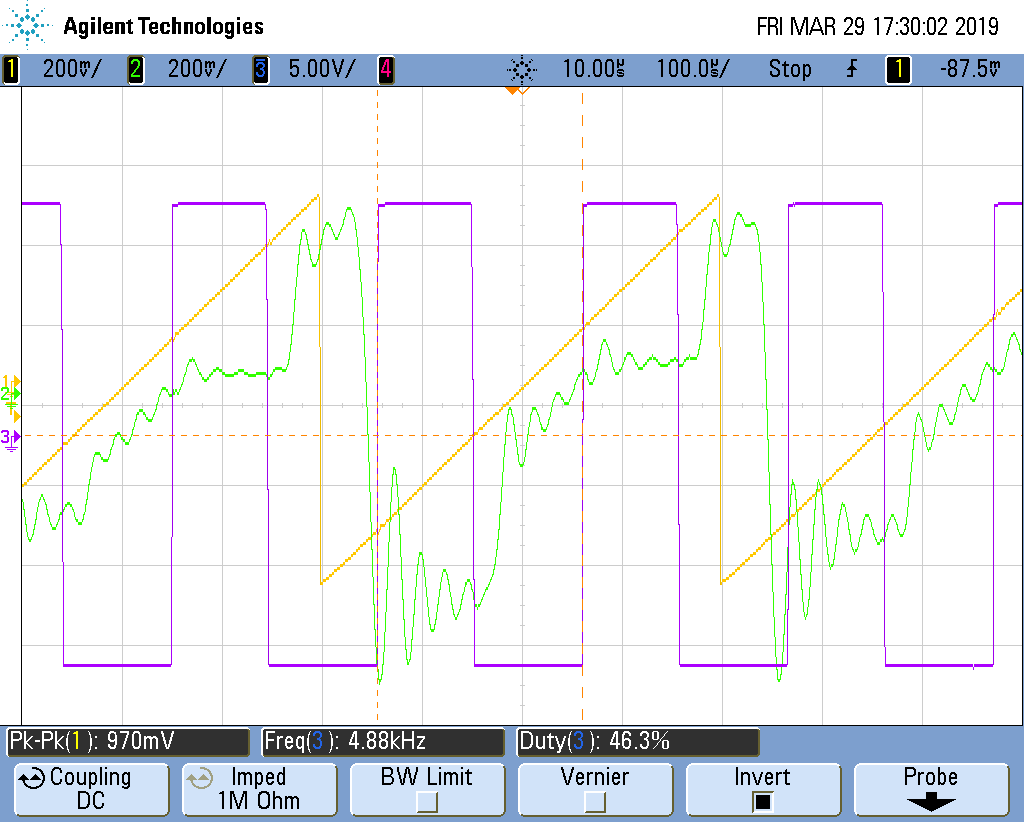
\includegraphics[scale=0.3]{Imagenes/yh_pt6d_cuad2}
\par\end{centering}
\caption{Señal muestreada con una señal de 20kHz.}
\end{figure}

\newpage

\section{Sample and Hold}

\subsection{Optimización}

Similar a la sección 1.1, utilizando el sample and hold , se calibraron
todas las partes de la placa par así poder obtener la menor distorción
posible con un óptimo $f_{s}\,y\,A$. Podemos observar el resultado
en las siguientes imágenes:

\begin{figure}[H]

\centering{}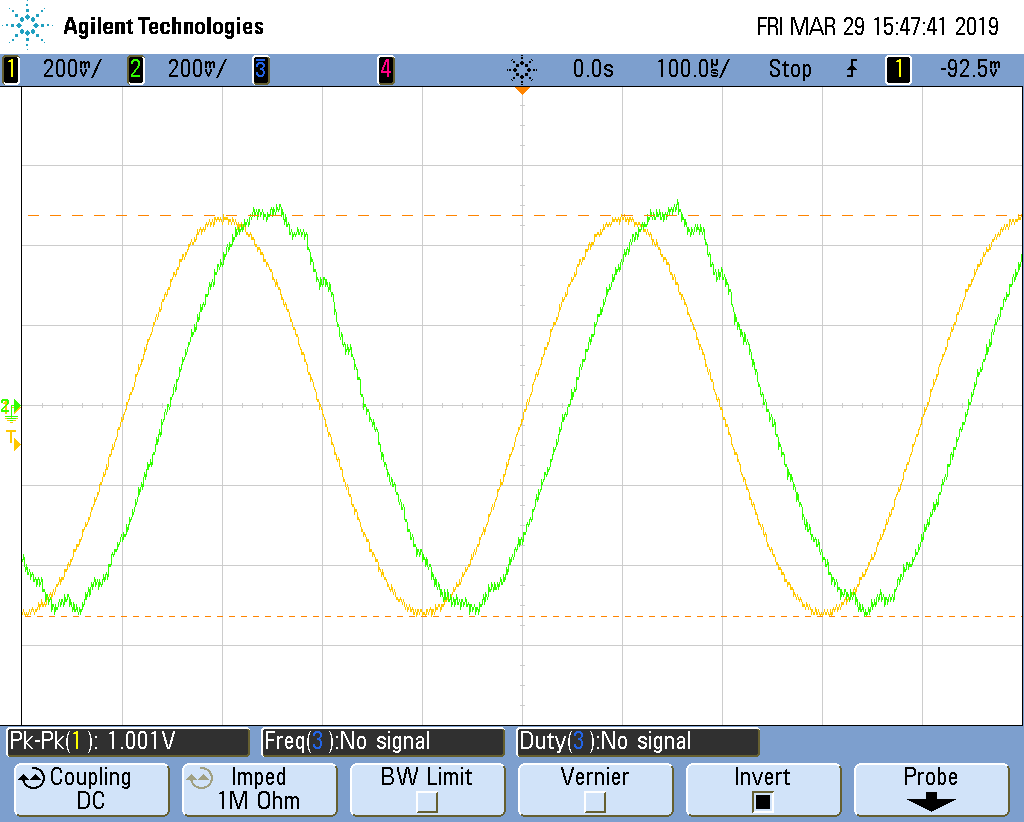
\includegraphics[scale=0.25]{Imagenes/syh_pto_asin3}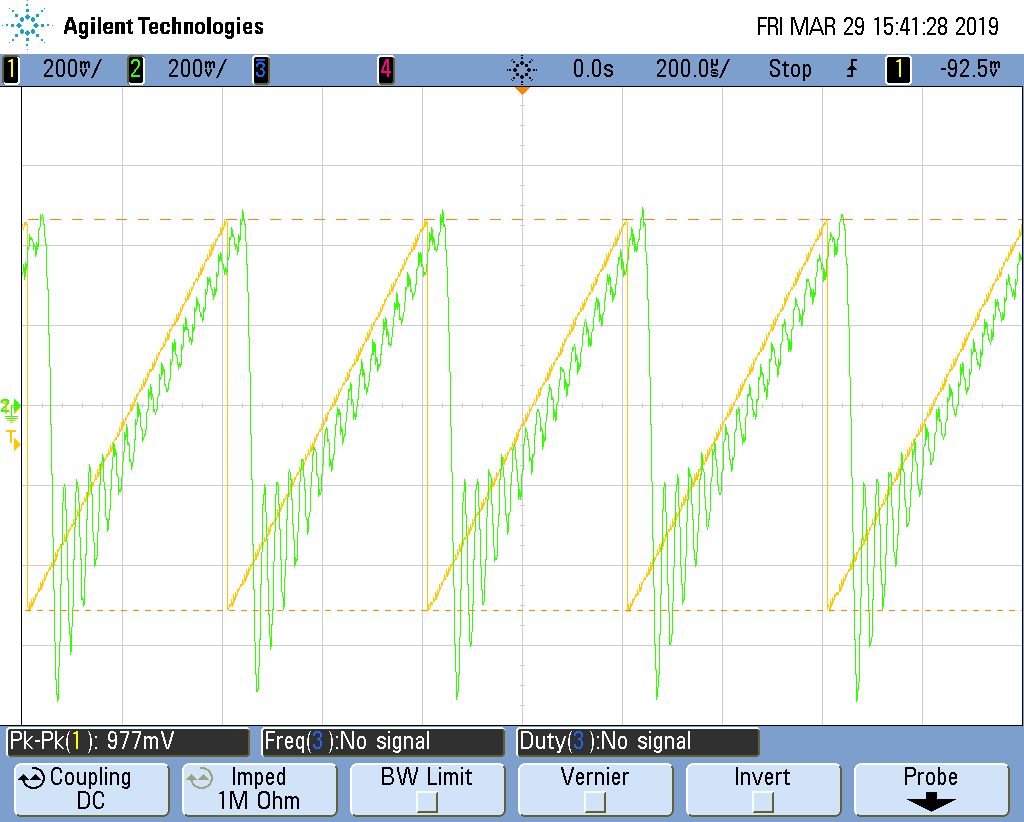
\includegraphics[scale=0.25]{Imagenes/syh_pto_adiente}\caption{De izq a der: salida (verde) de la placa con $X_{a}$; salida con
$X_{b}$}
\end{figure}

Para la señal $X_{a}$, los valores óptimos que se obtuvieron fueron:
$f_{s}:[83;307](kHz)$midiendo en el máximo de ese intervalo, $DC=34.5\%,$$A:(0;2]$(Vpp)
midiendo para $A=1V_{pp}$.

Para la señal $X_{b}$, los valores óptimos obtenidos fueron: $f_{s}:[91;307](kHz)$
midiendo en la frecuencia de 290kHz (pertenceciente a ese intervalo),
$DC=[30;47.5](\%)$, $A:(0;2]$(Vpp) midiendo para $A=1V_{pp}$.

FALTA POTENCIA Y DESARROLLO MATEMATICO???

\subsection{Cambios en la $f_{in}$ y en la $f_{s}$}

\subsubsection{$f_{in}<\frac{f_{p}}{2}$,$f_{s}=f_{a}$}

Para este caso, se exitó a la placa con una señal $X_{a}$, con la
diferencia respecto al punto anterior de que ahora el rango de $f_{in}=(0;17.5]$(kHz)
y la $f_{s}=68kHz.$Con el nuevo intervalo de $f_{in}$, finalmente
se eligió $f_{in}=500Hz.$ El duty cycle utilizado fue de 47.6\%.

Para la señal $X_{b}$, por otra parte el rango de $f_{in}$ pasó
a ser $f_{in}=(0;11.5]$(kHz) y la $f_{s}$ mantuvo su valor de $68kHz.$Con
el nuevo intervalo de $f_{in}$, finalmente se eligió $f_{in}=11.5kHz.$
El duty cycle utilizado también fue de 47.6\%.

Los resultados se ven plasmados en la siguiente image:

\begin{figure}[H]

\begin{centering}
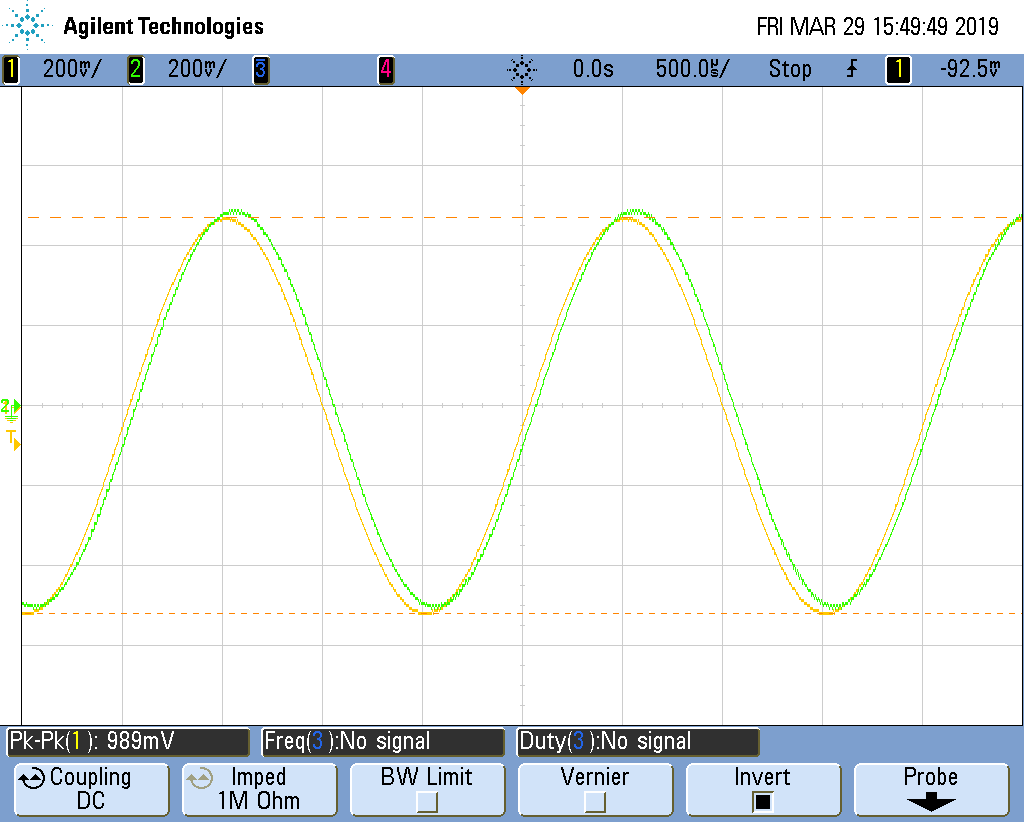
\includegraphics[scale=0.25]{Imagenes/syh_pto_bsin}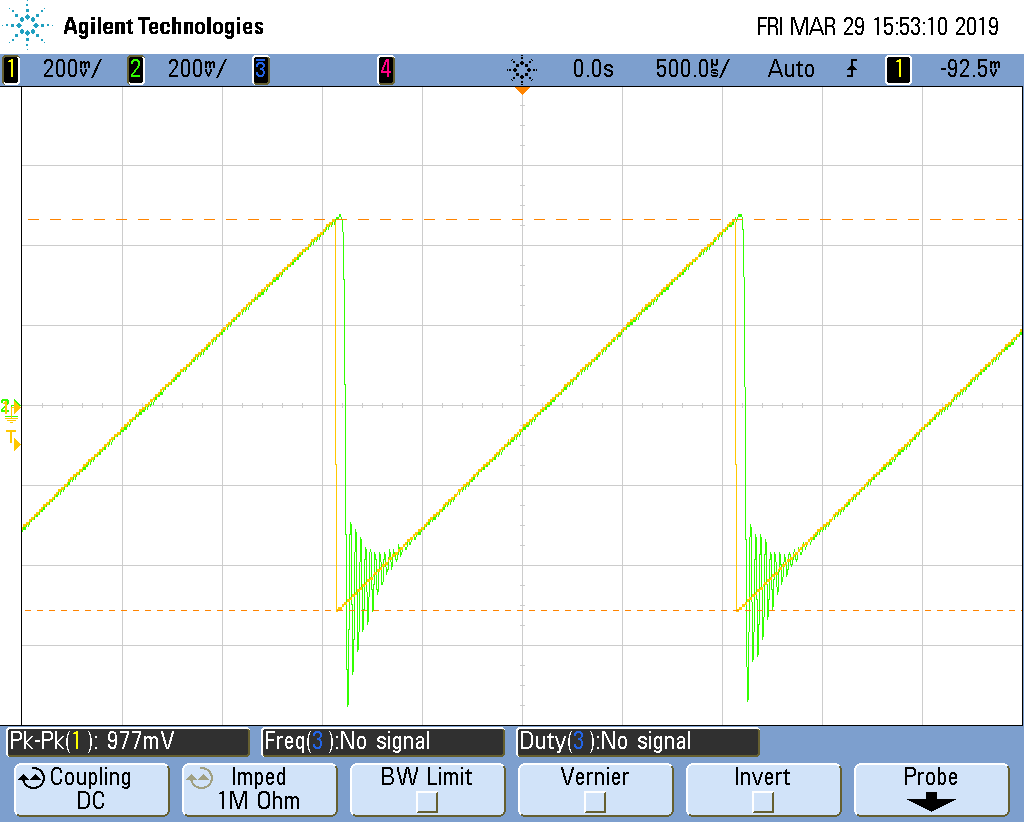
\includegraphics[scale=0.25]{Imagenes/syh_pto_bcuad_1}\caption{De izquierda a derecha: señal $X_{a}$y señal $X_{b}$.}
\par\end{centering}
\end{figure}


\subsubsection{$f_{in}=f_{a}$}

Para este punto, nuevamente, tanto a la señal $X_{a}$ como $X_{b}$,
se las estableció con una frecuencia $f_{in}=68kHz$. Para la frecuencia
de muestreo, se optó por utilizar la máxima posible, es decir $f_{s}=313kHz.$Para
ambas señales, se mantuvo el mismo duty cycle de 48\%. Los resultados
pueden ser apreciados en la siguiente imagen:

\begin{figure}[H]

\begin{centering}
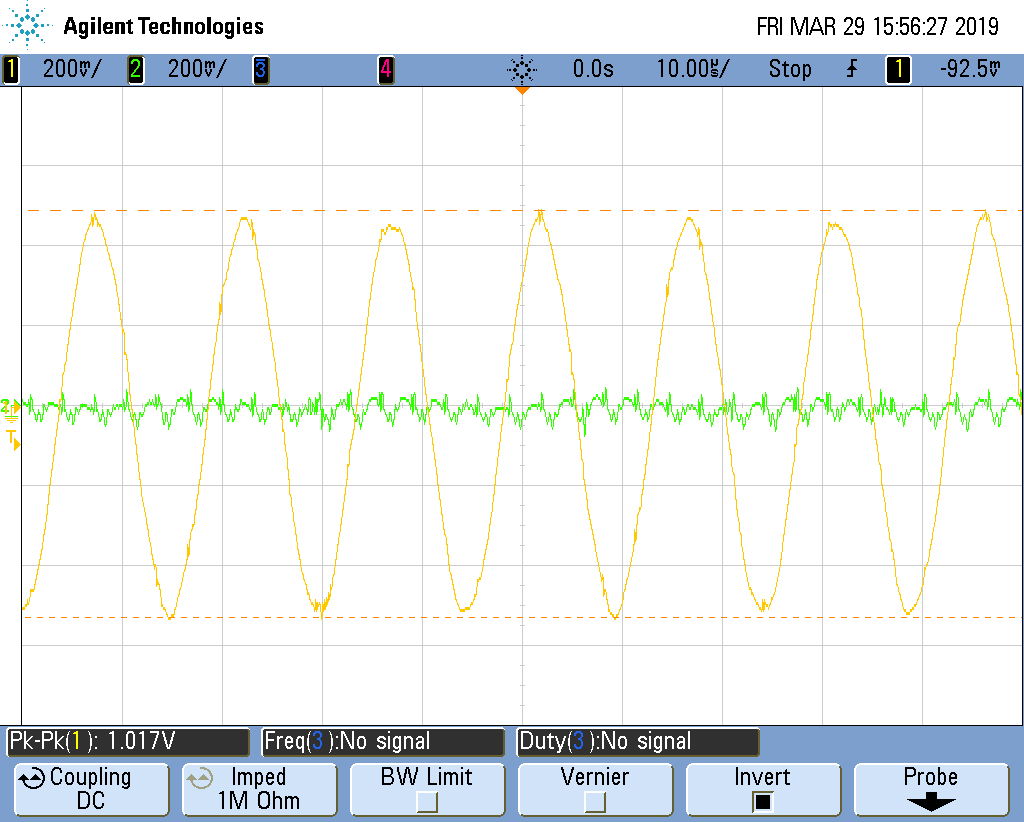
\includegraphics[scale=0.25]{Imagenes/syh_pto_bsin_67k}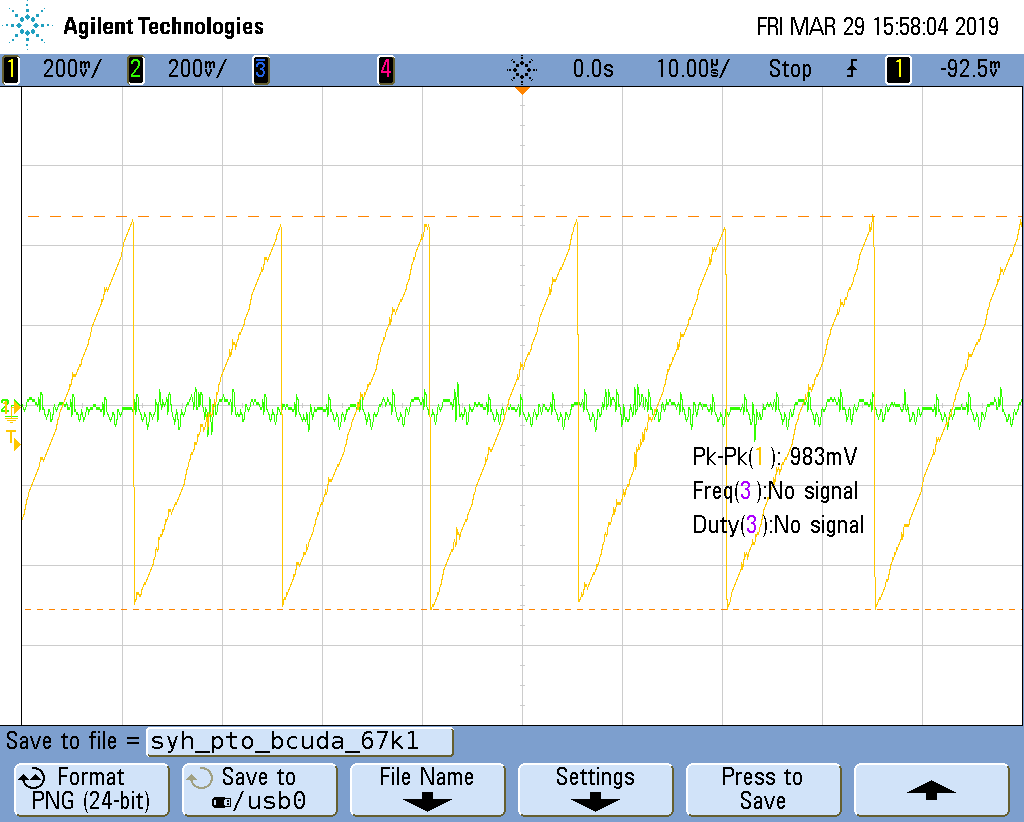
\includegraphics[scale=0.25]{Imagenes/syh_pto_bcuda_67k1}\caption{De izquierda a derecha: señal $X_{a}$y señal $X_{b}$.}
\par\end{centering}
\end{figure}


\subsection{$f_{in}=f_{s}\protect\leq f_{p}$}

Para este caso, igual que para su par con llave analógica, solamente
se exito al circuito con la señal $X_{a}$ con la particularidad que
la frecuencia de la señal coincide con la frecuencia de sampleo. Para
ello, se optó por utilizar $f_{in}=f_{s}=10kHz$ y un DC de 47.1\%.
La salida resultante se aprecia a continuación:

\begin{figure}[H]

\begin{centering}
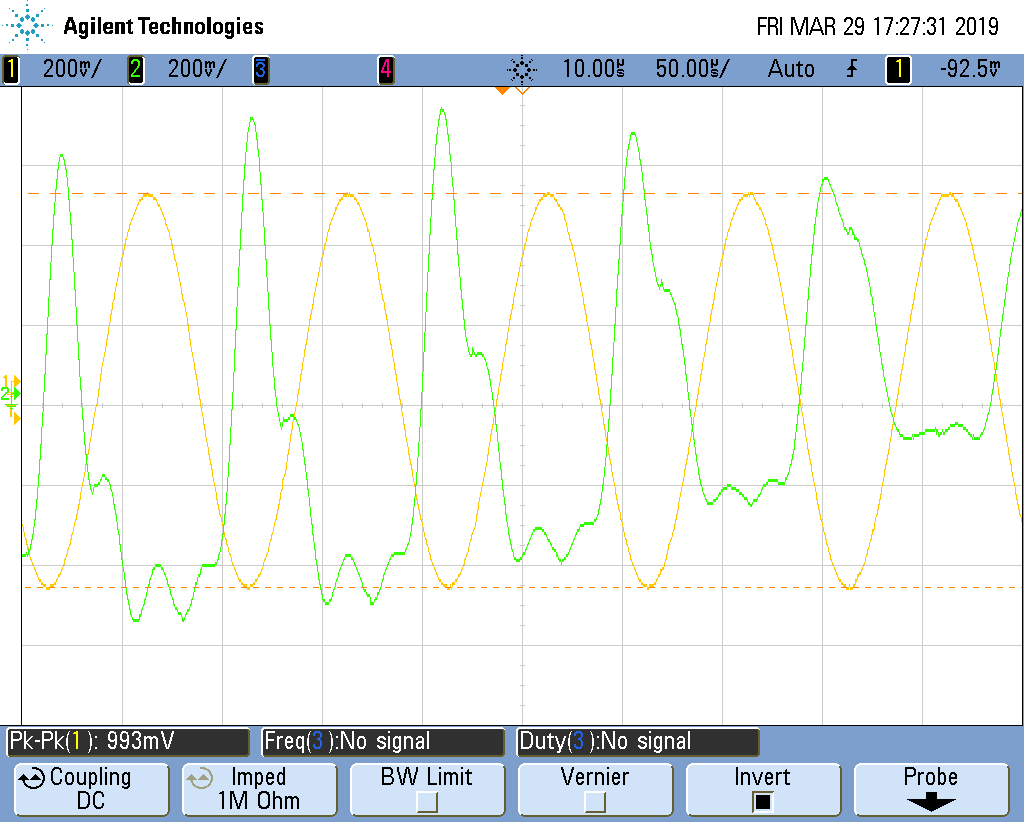
\includegraphics[scale=0.3]{Imagenes/yh_pt6c_sin2}\caption{Señal $X_{b}$ con frecuencia de muestreo igual a la de la señal.}
\par\end{centering}
\end{figure}


\subsection{Aliasing}

Para esta úlitma medición con la llave analógica, se exitó al circuito
con la señal $X_{b}$ variando su frecuencia $f_{in}$ de manera tal
de poder encontrar a qué frecuencia comienzan a aparecer problemas
de aliasing. Configurando la señal a una $f_{in}=2.5kHz,$observamos
que el efecto de aliasing aparece cuando la señal $f_{s}<6kHz$. Podemos
ver los efectos en la siguiente imagen:

\begin{figure}[H]
\begin{centering}
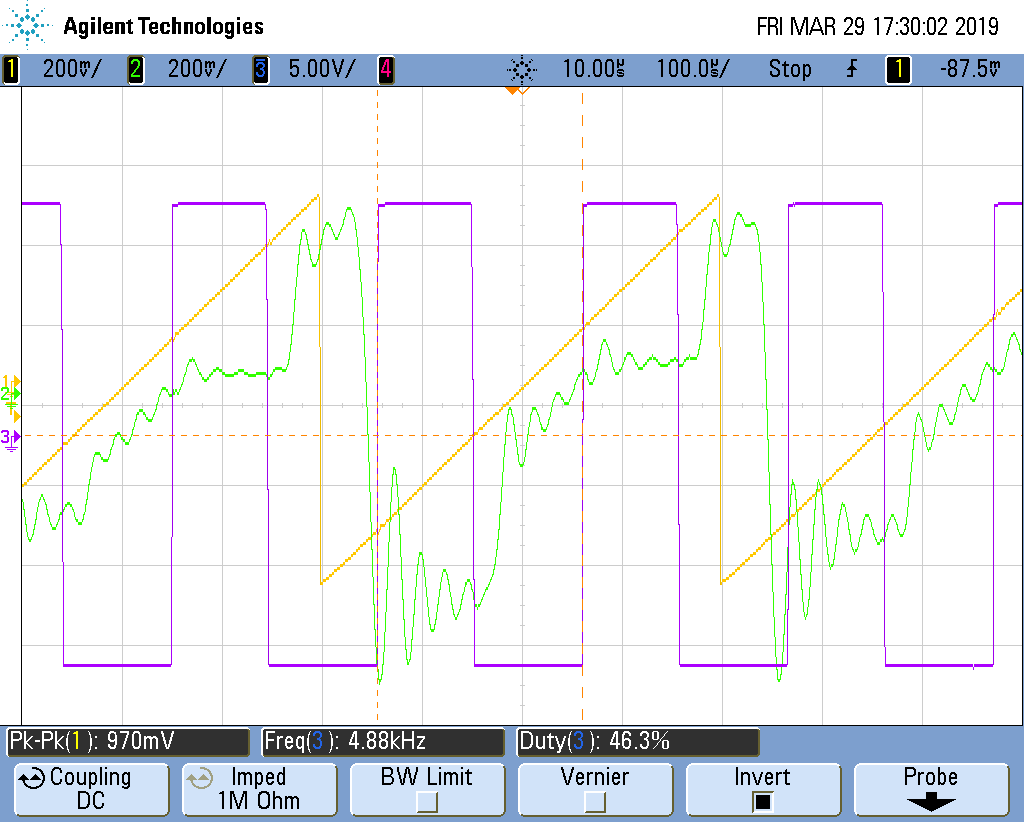
\includegraphics[scale=0.3]{Imagenes/yh_pt6d_cuad2}
\par\end{centering}
\caption{Señal muestreada con una señal de 20kHz.}
\end{figure}
\end{document}
